% chapter7_implementation.tex

\section{Chapter Overview}
This chapter describes the implementation of \textbf{RootLens} in detail, covering the development environment, technology stack, and the key implementation decisions for each system component. The chapter highlights the implementation of the \textbf{rule-based engine}, the ML model training and loading pipeline, the event processing architecture, and the React dashboard. Challenges encountered during implementation and their resolutions are discussed candidly, as these represent significant engineering lessons.

\section{Development Environment Setup}
Development was conducted on an Apple M-series MacBook (16\,GB RAM, macOS Sonoma) using Go 1.25, Python 3.9 (via pyenv), Node.js 20 LTS, Docker Desktop, and Minikube 1.33 (4 vCPUs, 8\,GB RAM) with KEDA 2.15 and kubebuilder. Version control used Git with a feature-branch workflow.

\section{Technology Selection}
This section justifies the selection of tools, frameworks, and programming languages used for the development of RootLens.

\subsection{Technology Stack}
The Go backend uses the standard library HTTP server, the client-go library for Kubernetes event streaming, and the controller-runtime framework for the Operator reconciliation loop. The React dashboard uses functional components with hooks, Recharts for data visualisation, and Axios for API communication. Kubernetes deployment uses kubebuilder for Operator scaffolding and Helm for installing cluster dependencies.

\subsection{Programming Languages}
\textbf{Go 1.25} was selected for the backend due to its native concurrency model (goroutines and channels), which is essential for handling multiple concurrent Kubernetes Watch streams with minimal memory overhead. Go's compiled binaries produce lightweight container images ($\sim$15\,MB), reducing cold start times in Kubernetes deployments. \textbf{Python 3.9} was used for the ML service, as scikit-learn Random Forest models are natively supported and the ecosystem provides mature tools for feature engineering and model serialisation. \textbf{JavaScript (ES2024)} was used for the React dashboard frontend.

\subsection{Development Frameworks}
\textbf{Flask} was selected for the ML service due to its lightweight HTTP interface with minimal overhead, suitable for serving ML predictions. \textbf{React 19} was chosen for the dashboard as it provides a component-based architecture with hooks for state management, enabling responsive real-time data visualisation. \textbf{Kubebuilder v4} was used for scaffolding the Kubernetes Operator, following the standard controller-runtime reconciliation pattern.

\subsection{Libraries and Toolkits}
Key libraries include: \textbf{client-go} for Kubernetes API interaction, \textbf{scikit-learn} for Random Forest model training and inference, \textbf{Recharts} for dashboard data visualisation, \textbf{Axios} for HTTP communication, and \textbf{gorilla/mux} for HTTP routing in the Go API. Model serialisation uses Python's \textbf{joblib} library for efficient persistence of trained models and scalers.

\subsection{Integrated Development Environments}
Development was conducted using \textbf{Visual Studio Code} with Go, Python, and React extensions for language support, debugging, and linting. \textbf{Kubernetes Lens} was used for cluster monitoring and debugging during development and testing.

\subsection{Summary of Technology Selection}
\begin{table}[H]
\centering
\begin{tabularx}{\textwidth}{|l|X|X|}
\hline
\textbf{Category} & \textbf{Technology} & \textbf{Justification} \\ \hline
Backend Language & Go 1.25 & Native concurrency, lightweight binaries \\ \hline
ML Language & Python 3.9 & scikit-learn ecosystem, mature ML tooling \\ \hline
Frontend & React 19 & Component architecture, real-time updates \\ \hline
ML Framework & Flask + scikit-learn & Lightweight serving, native RF support \\ \hline
Orchestration & Kubernetes + KEDA & Target platform for the research \\ \hline
Operator & Kubebuilder v4 & Standard controller-runtime pattern \\ \hline
IDE & VS Code, K8s Lens & Multi-language support, cluster monitoring \\ \hline
\end{tabularx}
\caption{Technology Selection Summary}
\label{tab:tech_summary}
\end{table}

\section{System Implementation}

\subsection{Metrics Collection and Integration}
The metrics collection layer is implemented as concurrent goroutines launched at startup. The Kubernetes Event Watcher uses client-go's \texttt{Watch} mechanism (\textbf{adapted} from the official Kubernetes client library documentation (Kubernetes Authors, 2024)) to stream pod lifecycle events with RootLens-specific filtering and timestamp extraction. The KEDA state poller runs in a separate goroutine, polling the ScaledObject resource every 5 seconds and recording scaling events when desired replica count changes. The RabbitMQ metrics collector queries the Management API to capture queue depth at the moment of KEDA trigger detection.

\subsection{Event Processing Pipeline}
Event processing follows a producer-consumer pattern (\textbf{adapted} from standard Go concurrency idioms) using Go channels, with \textbf{novel} event correlation logic that matches events by pod UID across multiple concurrent API sources. A central \texttt{EventAggregator} correlates events from the same pod, assembles complete timing snapshots, and passes them to the RCA engine. Figure~\ref{fig:aggregator} shows the core aggregation logic.

\begin{figure}[H]
\centering
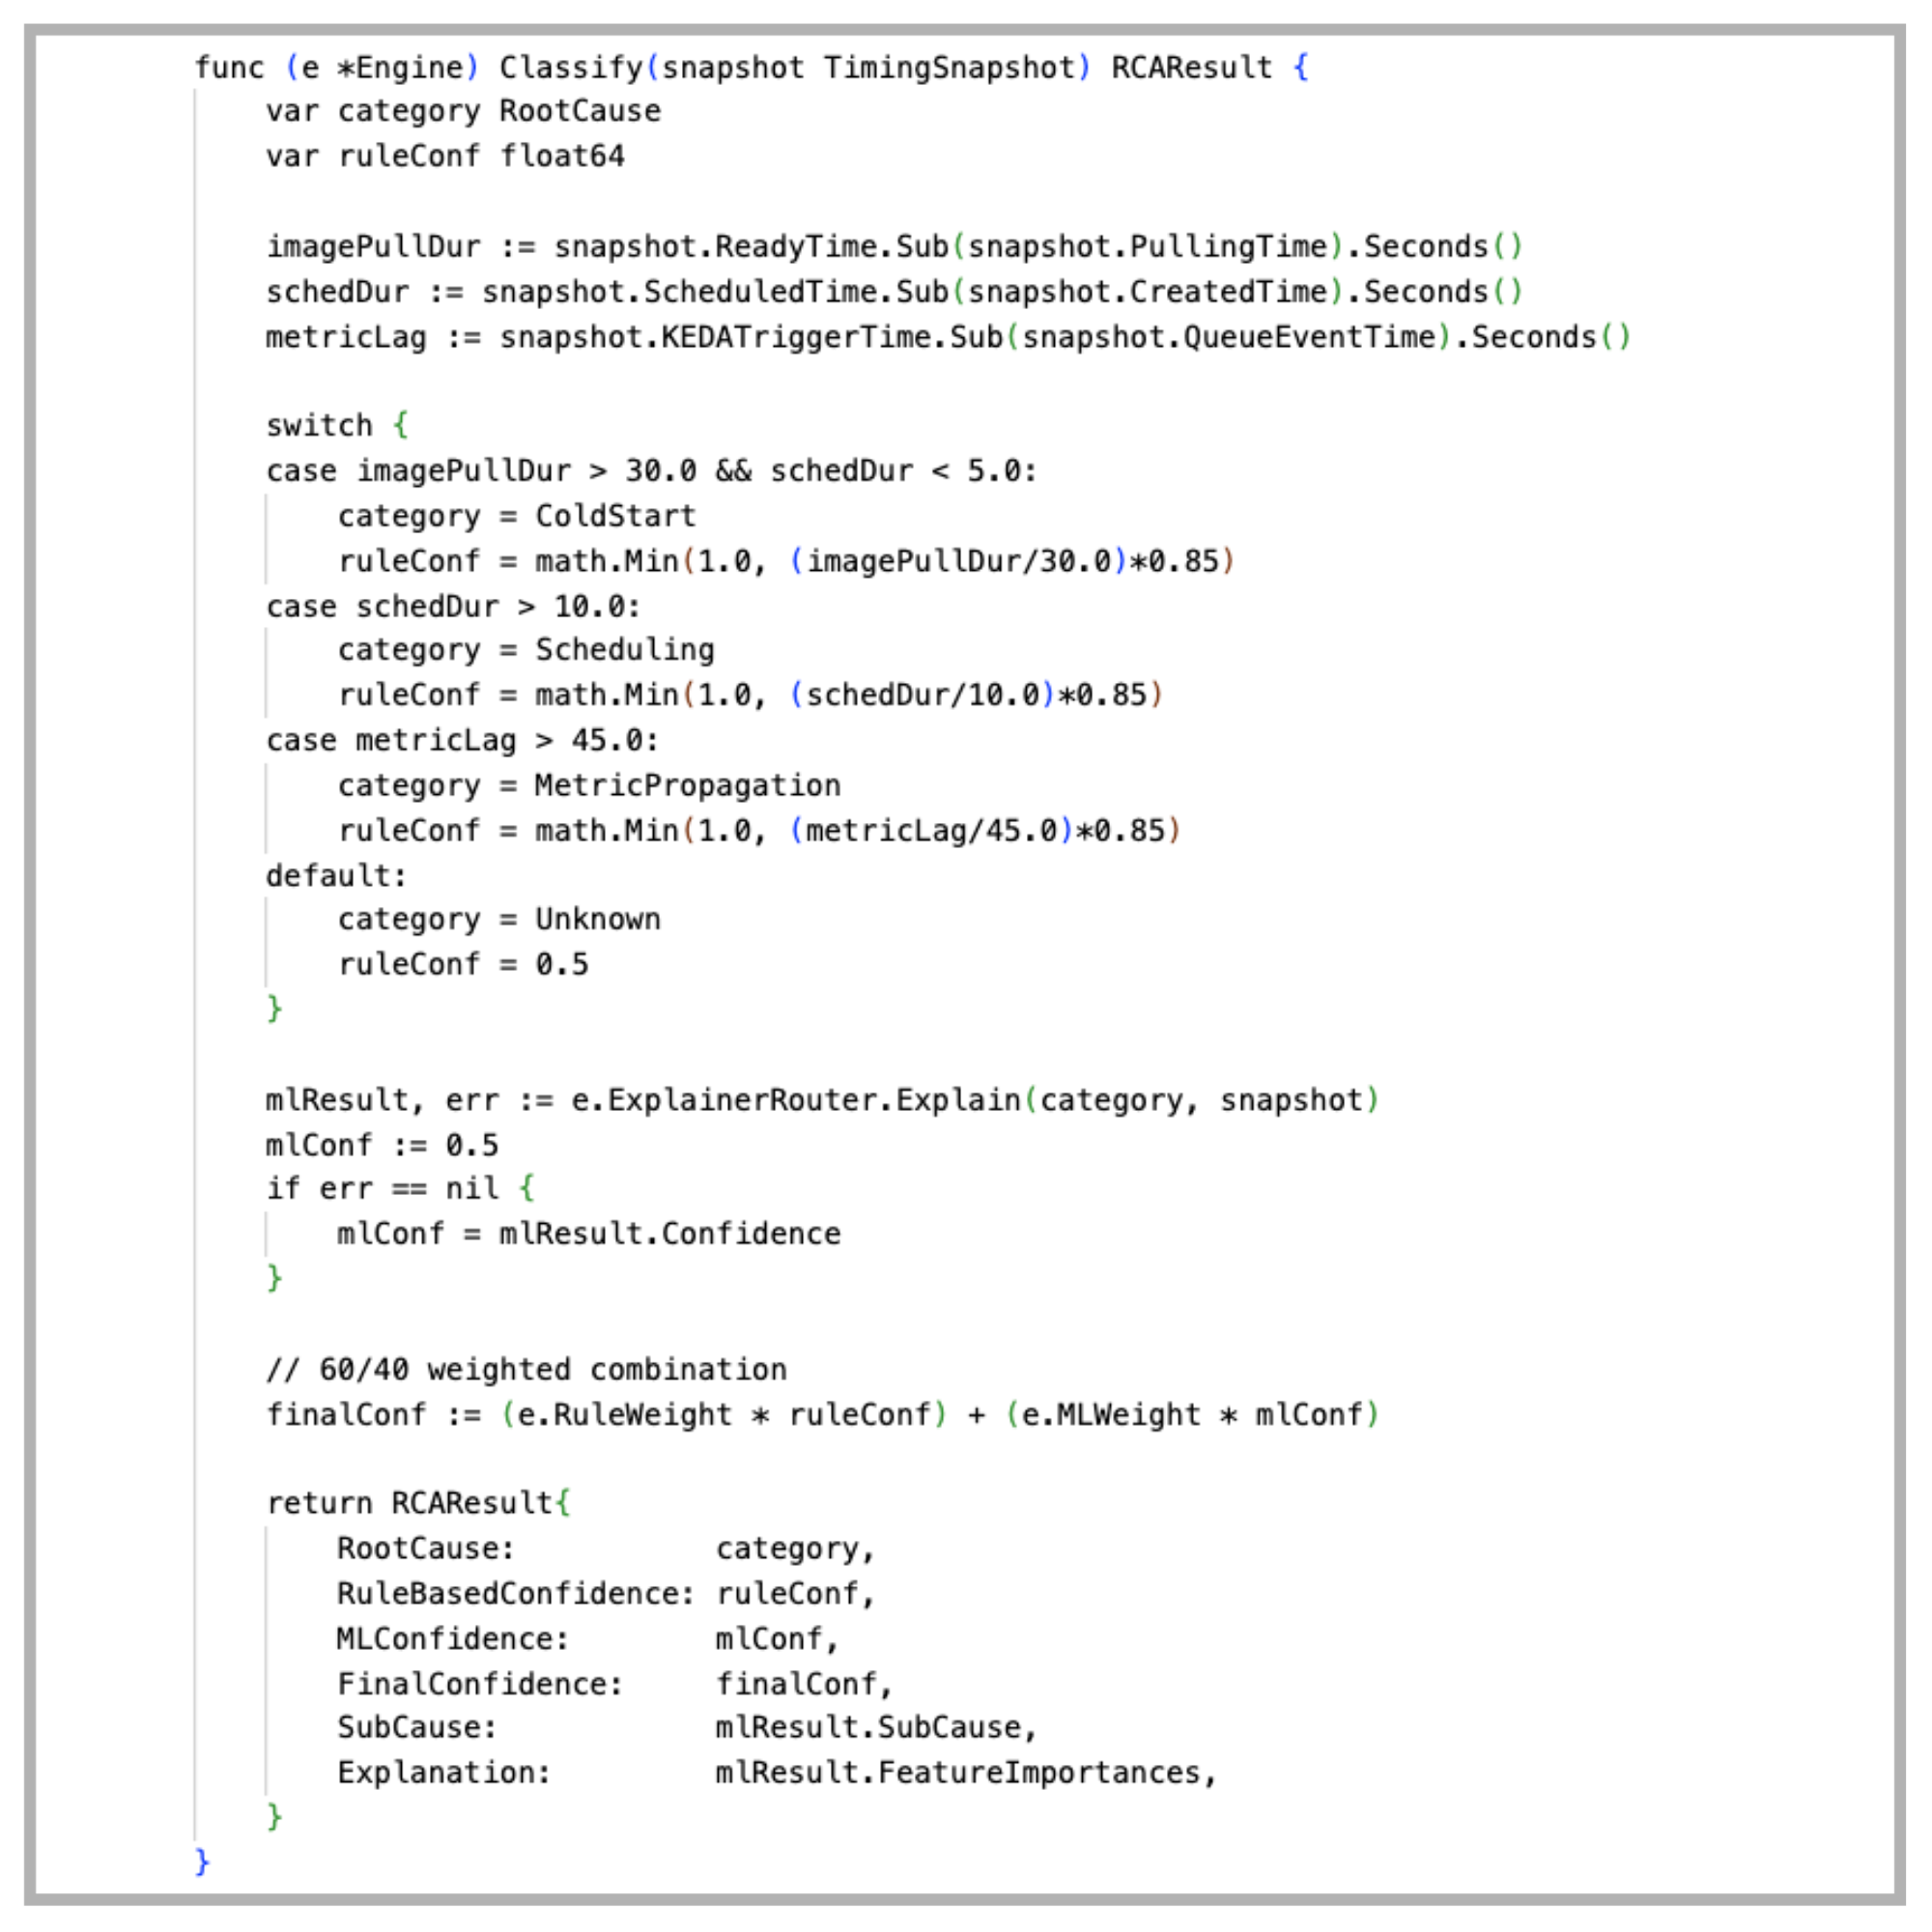
\includegraphics[width=0.85\textwidth]{thesis/assets/code_1.png}
\caption{Core Aggregation Logic}
\label{fig:aggregator}
\end{figure}

\subsection{RCA Logic Implementation}
The core classification logic is implemented in \texttt{pkg/rca/engine.go}. Figure~\ref{fig:classify_logic} shows the classification function and confidence combination.

\begin{figure}[H]
\centering
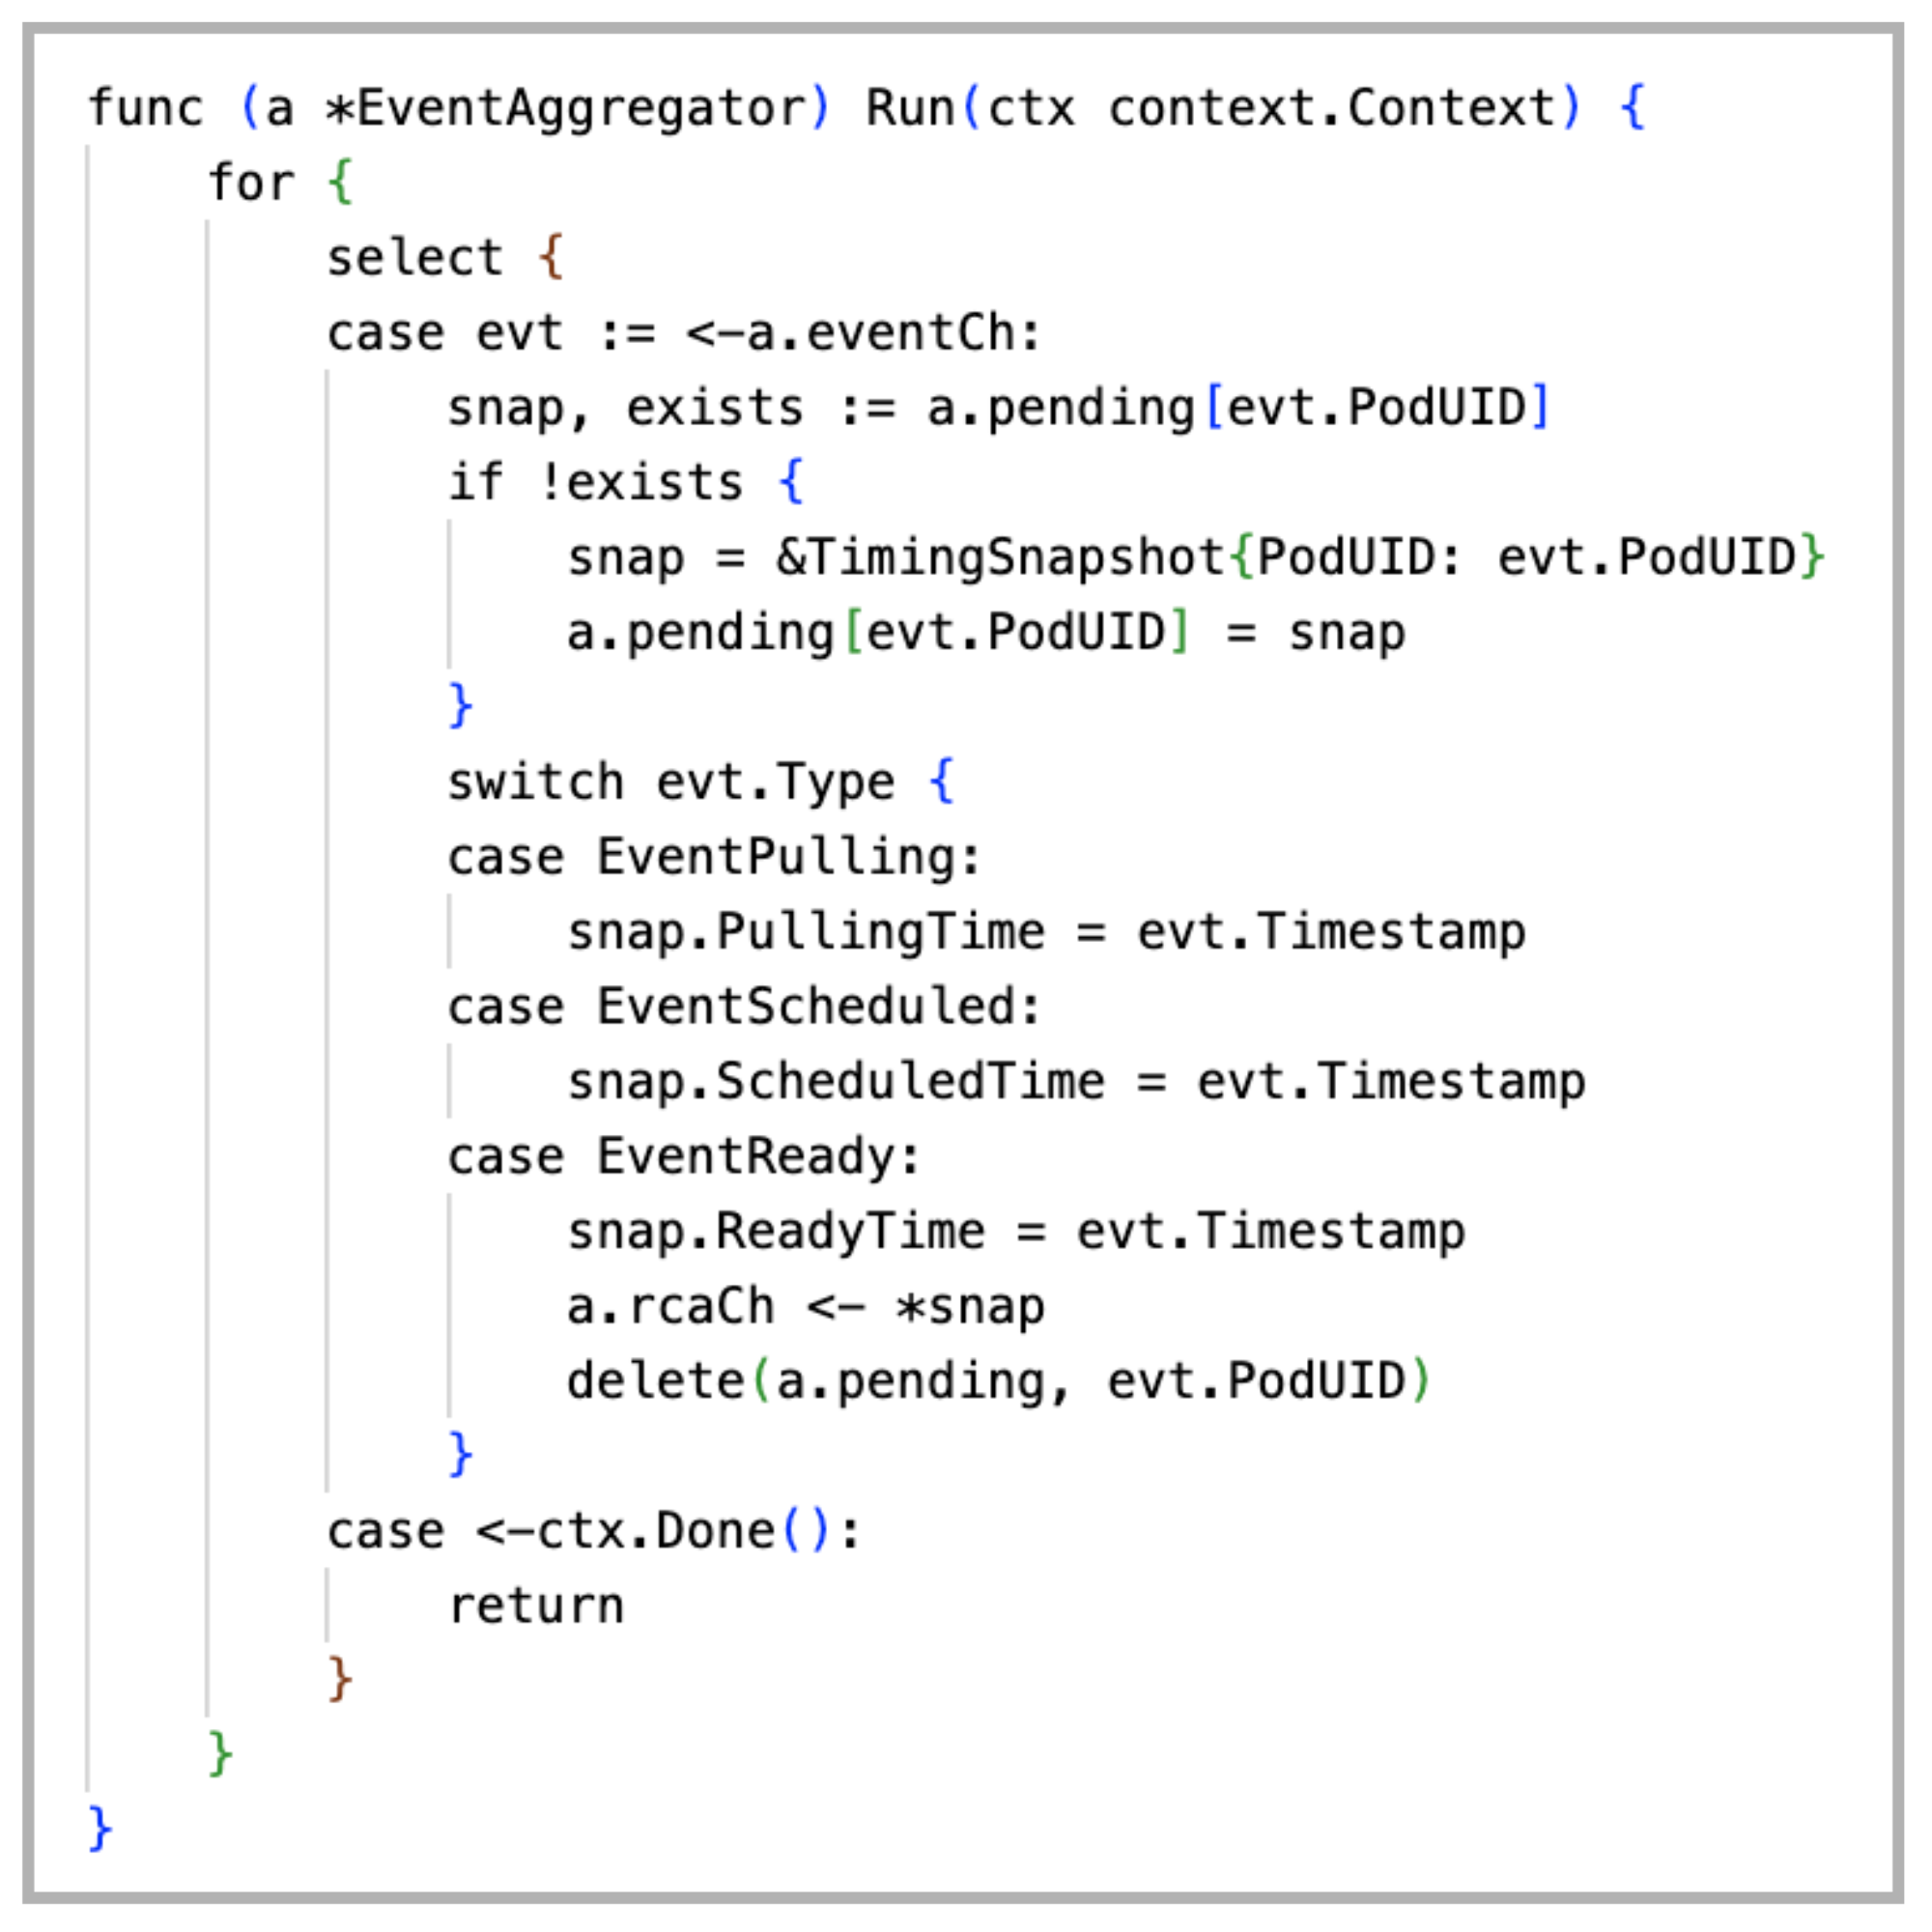
\includegraphics[width=0.85\textwidth]{thesis/assets/code_2.png}
\caption{Classification Logic}
\label{fig:classify_logic}
\end{figure}

This classification logic and the 60/40 confidence combination formula are \textbf{novel contributions} of this project, implementing the hybrid RCA pipeline designed in Chapter~6.

\subsection{ML Model Integration}

\textbf{Dataset Generation via Chaos Engineering:} Following the fault-injection methodology of Basiri et al. (2016), training data was generated by running 30 controlled experiments on Minikube (10 per root cause category). Each experiment injected a specific fault condition (e.g., rate-limited registry for cold start, CPU constraints for scheduling contention) and collected timing signals with ground-truth labels based on the known injected fault. Features were extracted per the category-specific definitions and saved as NumPy \texttt{.npz} files.

\textbf{Training Pipeline:} Three training scripts load the corresponding \texttt{.npz} files, apply a \texttt{StandardScaler}, and train a \texttt{RandomForestClassifier} with 100 estimators. Both the scaler and model are serialised as a wrapper dictionary. Figure~\ref{fig:train_snippet} shows the core training logic.

\begin{figure}[H]
\centering
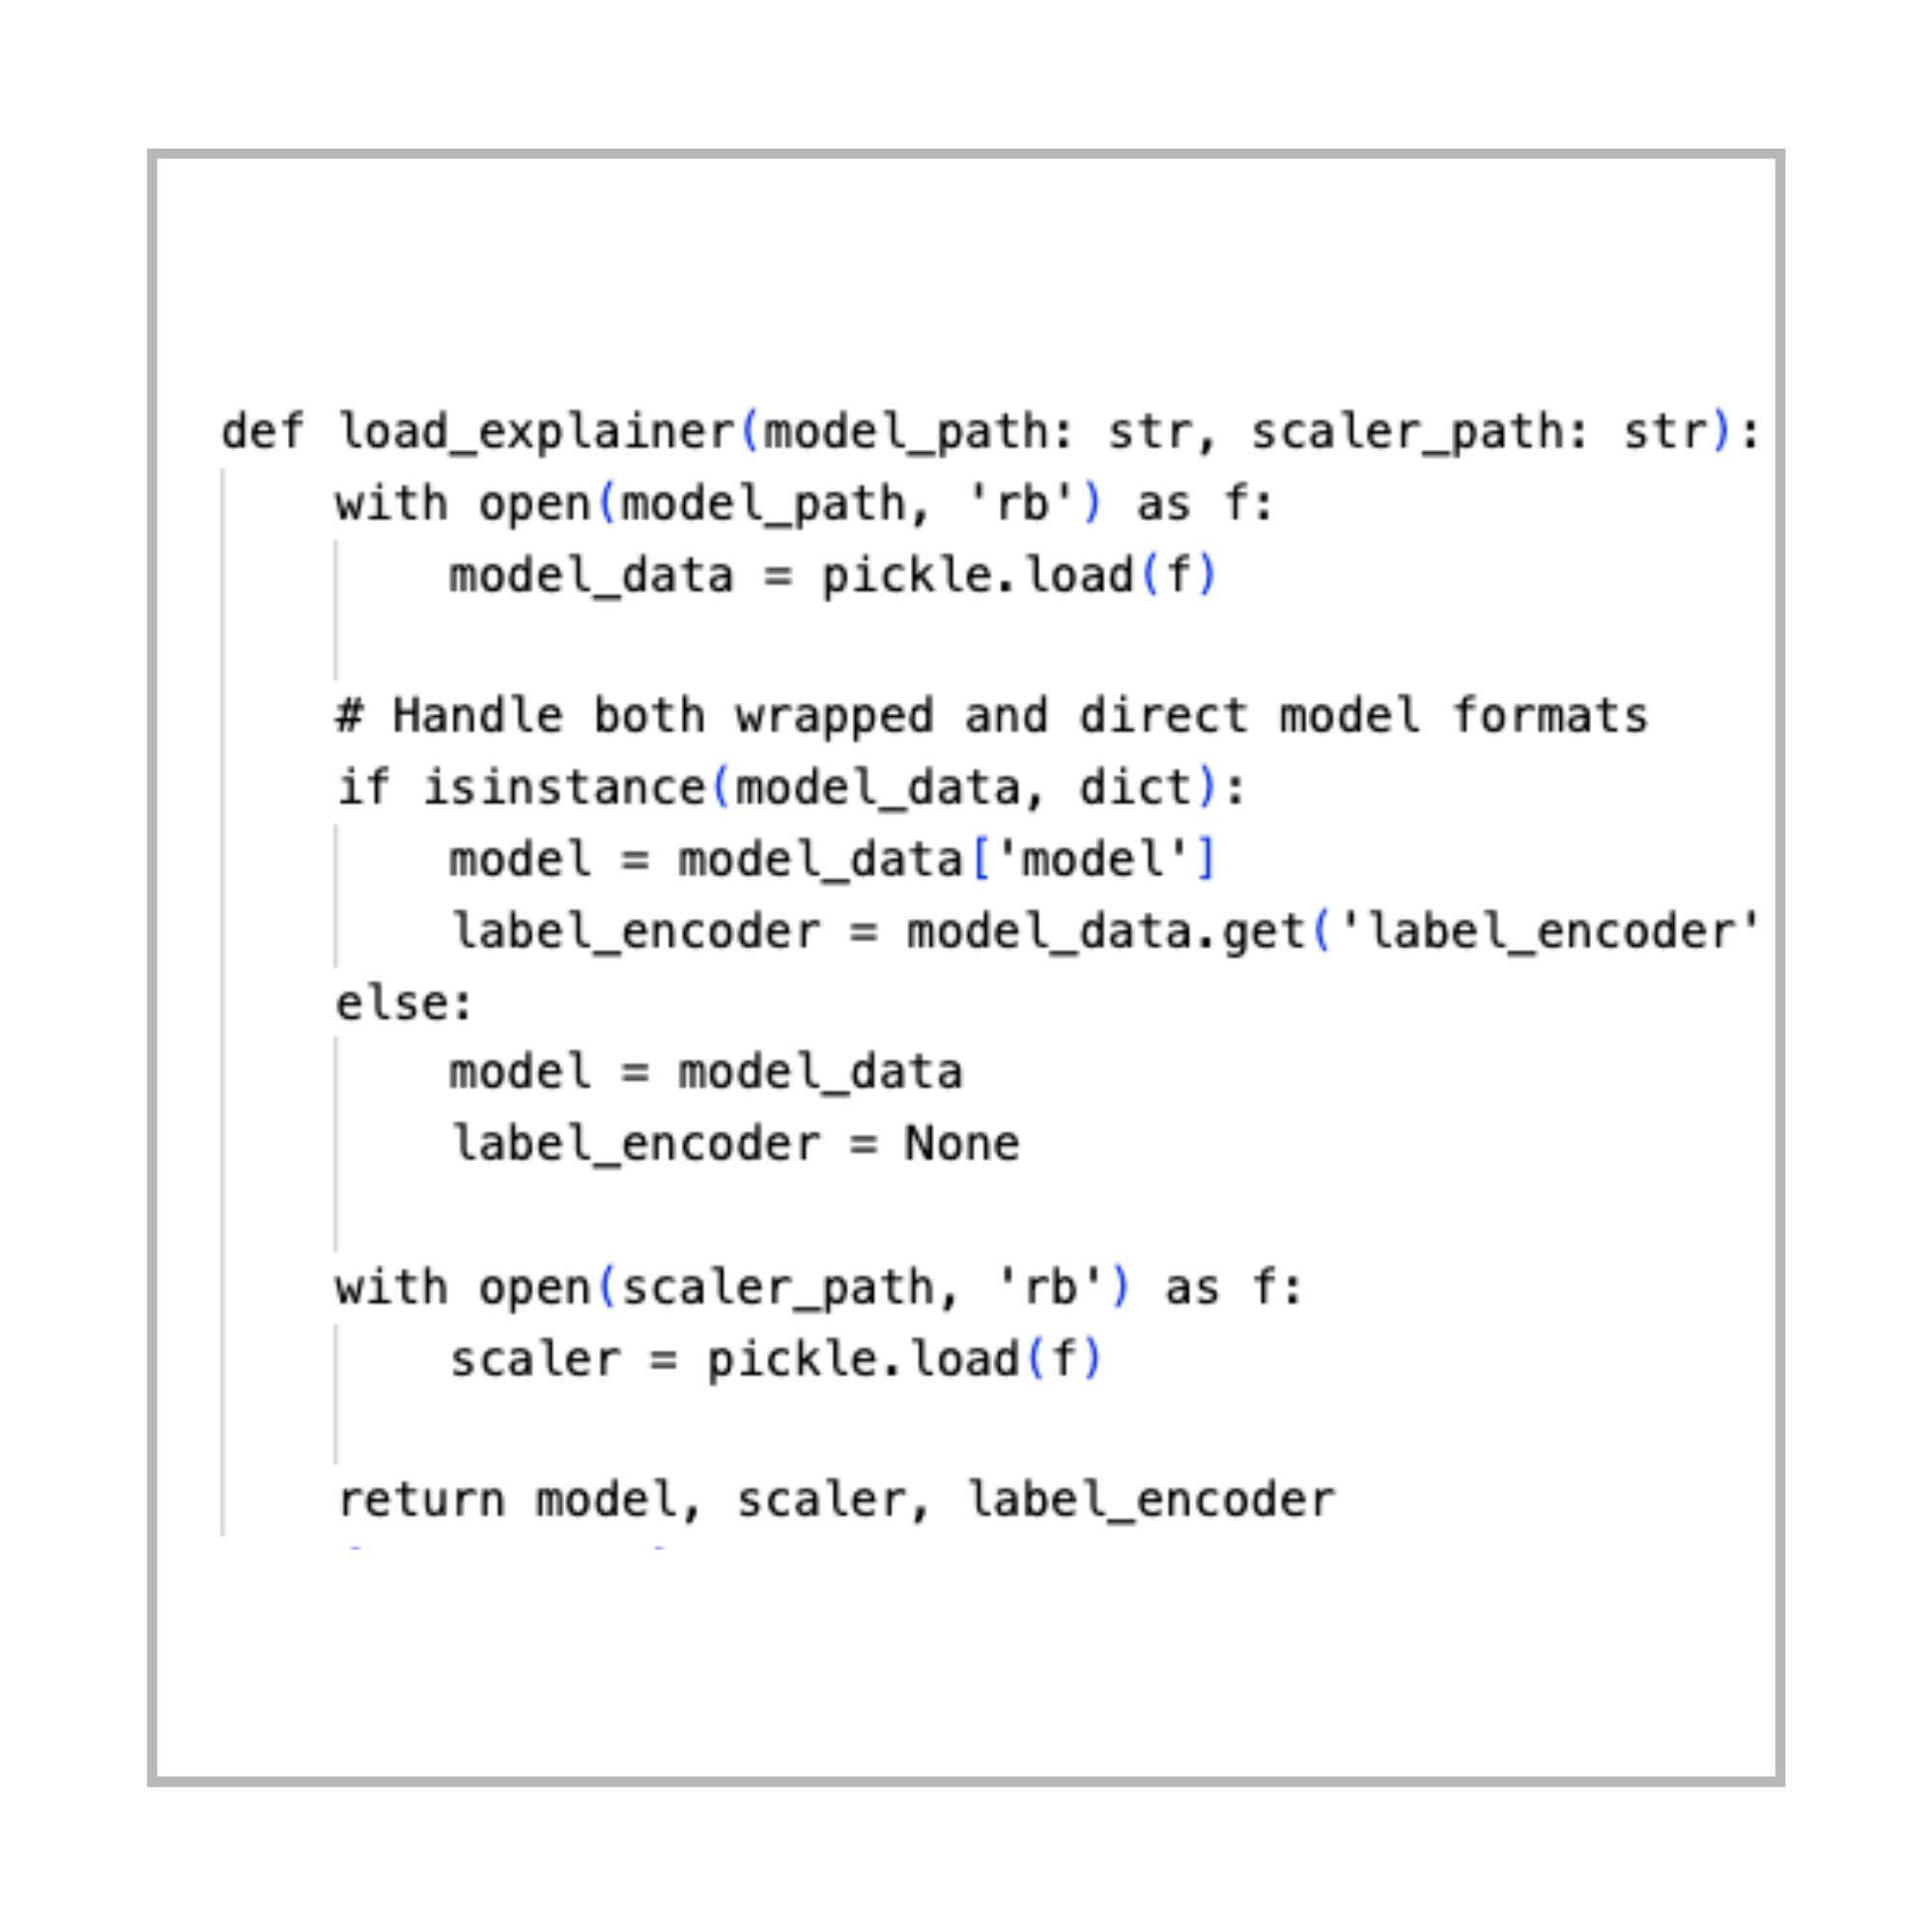
\includegraphics[width=0.85\textwidth]{thesis/assets/code_3.png}
\caption{Training Pipeline Code Snippet}
\label{fig:train_snippet}
\end{figure}

The training pipeline follows standard scikit-learn practice (Breiman, 2001), but the category-specific feature sets and wrapper serialisation format are \textbf{novel} to this project.

\textbf{Model Loading and Inference:} The model loading function handles both wrapped dictionary and direct model formats. When loading a saved model, the code checks \texttt{isinstance(model\_data, dict)} and extracts the model via \texttt{model\_data['model']} if wrapped. This wrapper-handling pattern was developed as a \textbf{novel solution} to the implementation challenge described in Section~7.8, where model serialisation inconsistencies caused runtime failures.

\section{UI Implementation (Additional Component)}
The React dashboard consumes the REST API JSON output, polling the latest result endpoint every 10 seconds. Recharts bar charts display feature importances, a confidence gauge renders the final score, and all error states are caught by the \texttt{ErrorBoundary} component. The dashboard is a convenience interface; the primary system output remains the JSON API response (see Appendix~B).

Figure~\ref{fig:website} shows the marketing website for RootLens. Additional pages are provided in the appendices.

\begin{figure}[H]
\centering
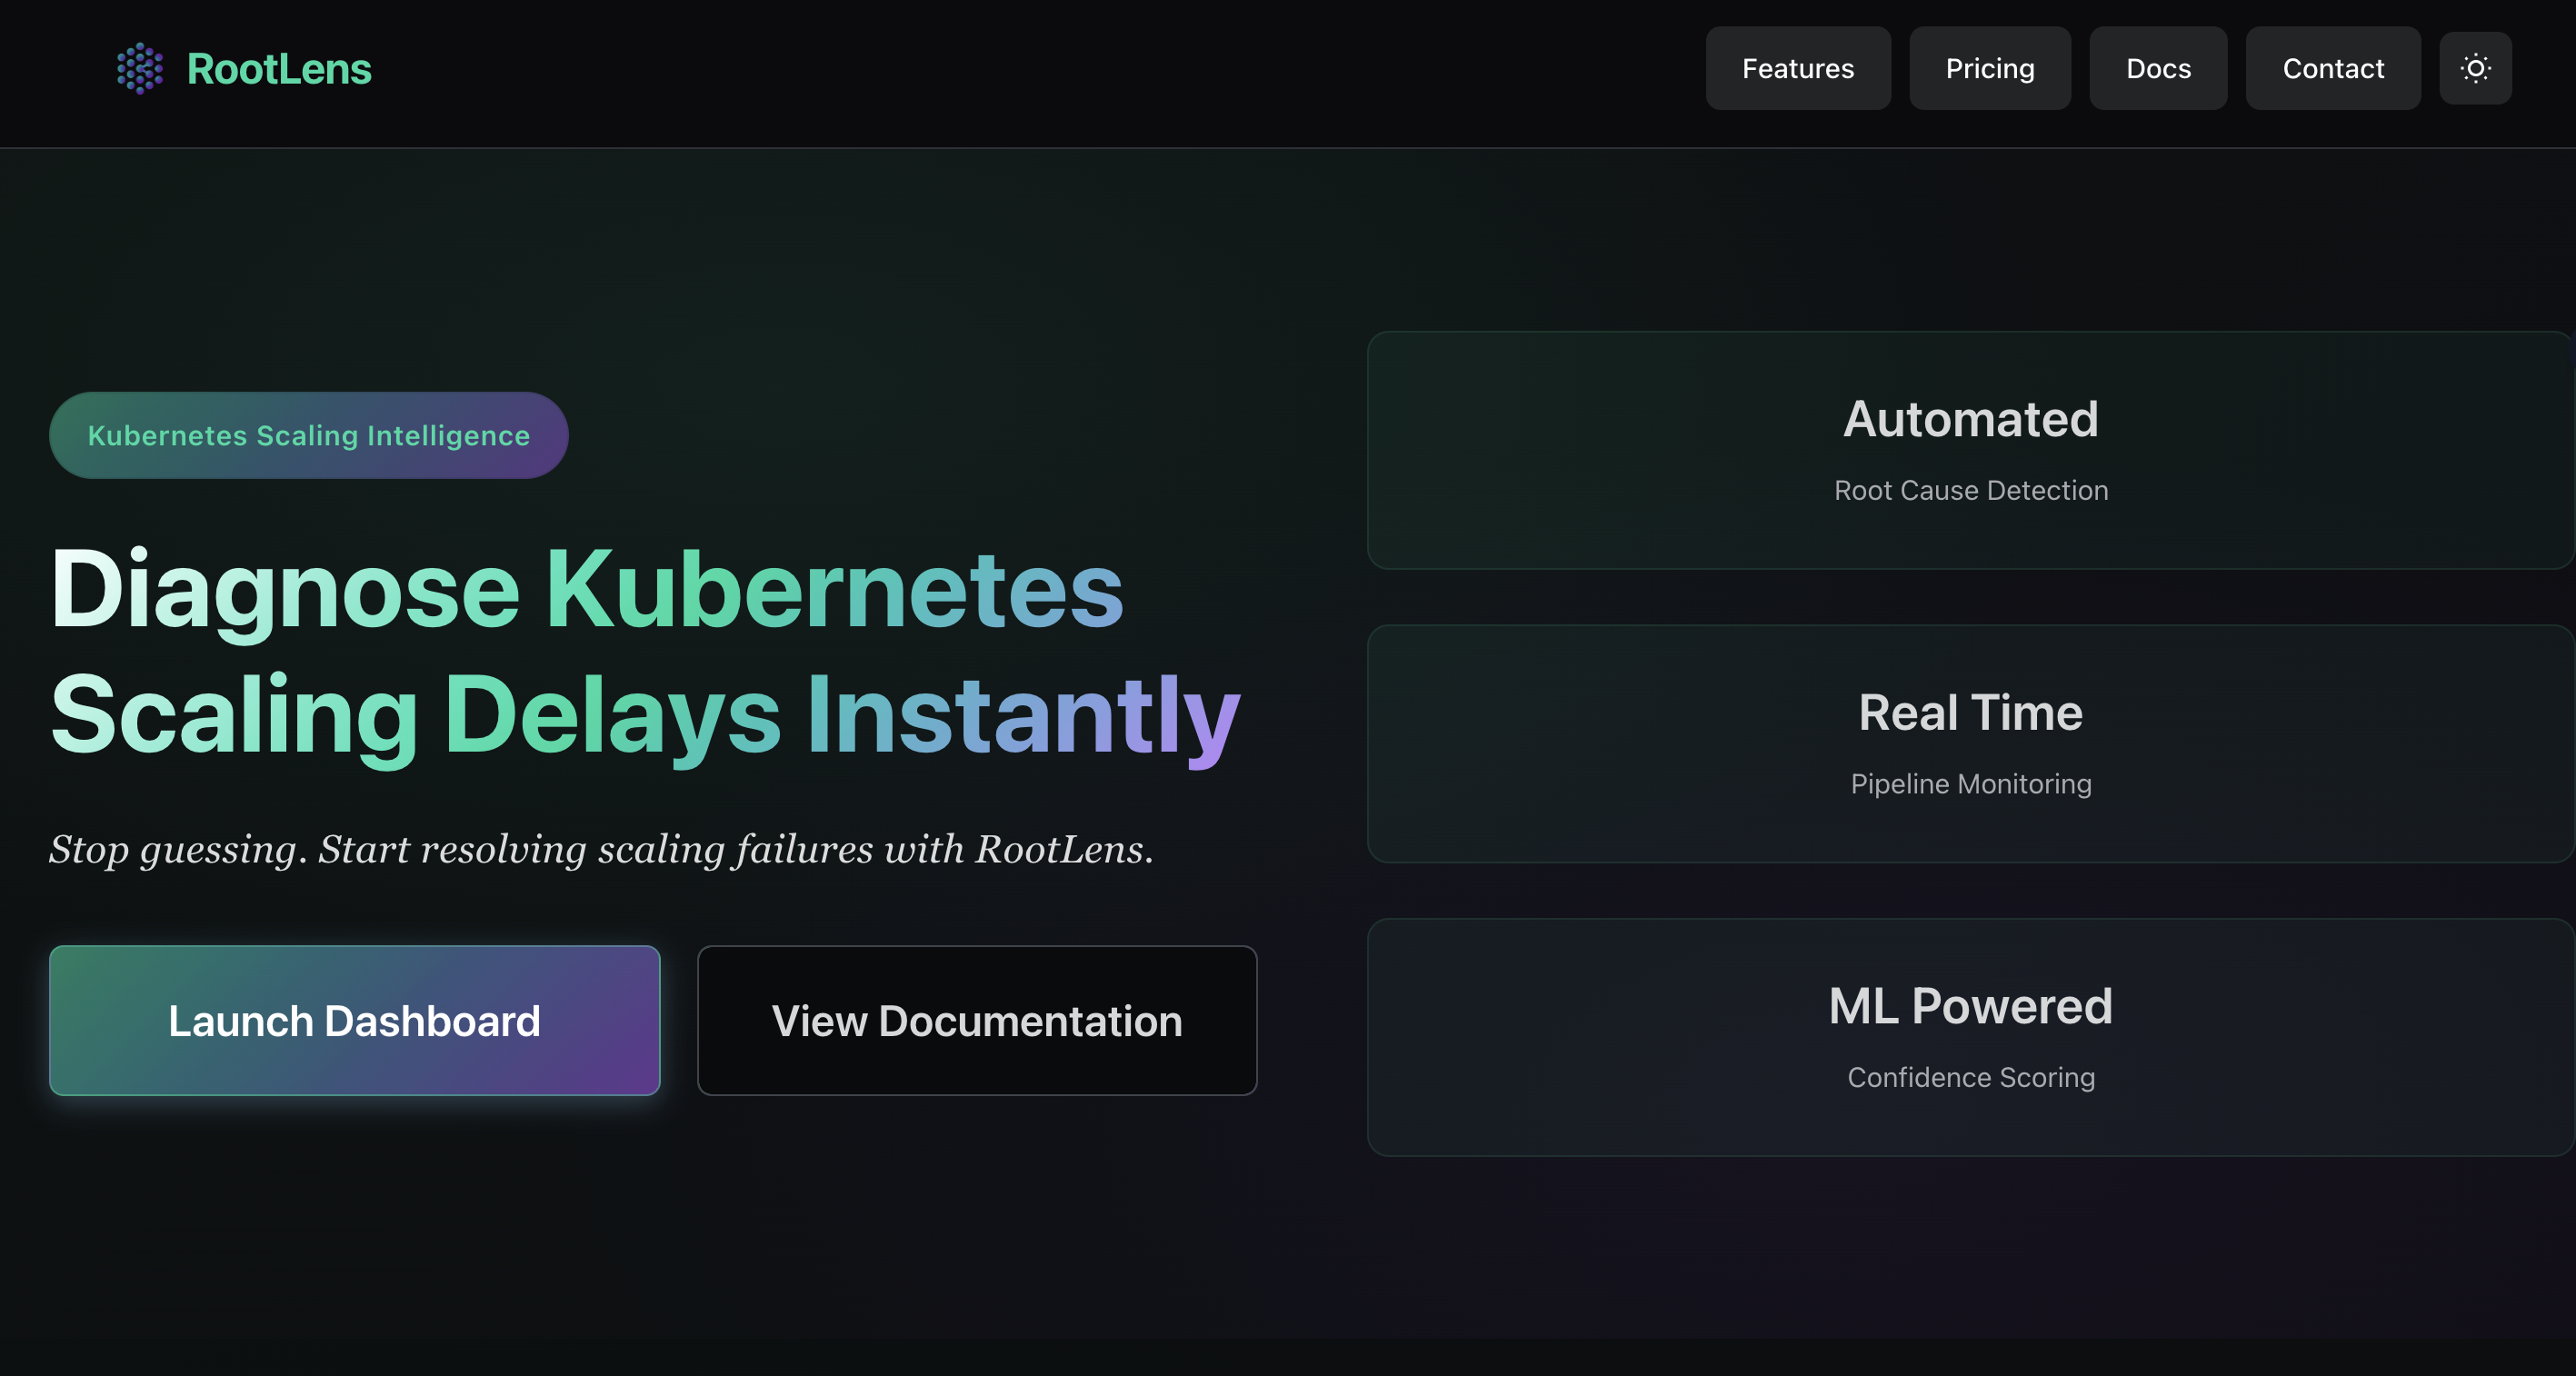
\includegraphics[width=0.95\textwidth]{thesis/assets/website.png}
\caption{RootLens Website}
\label{fig:website}
\end{figure}

Figure~\ref{fig:dashboard_overview} shows the dashboard overview page displaying the most recent RCA result, including root cause category, sub-cause, final confidence score, and the feature importance breakdown chart.

\begin{figure}[H]
\centering
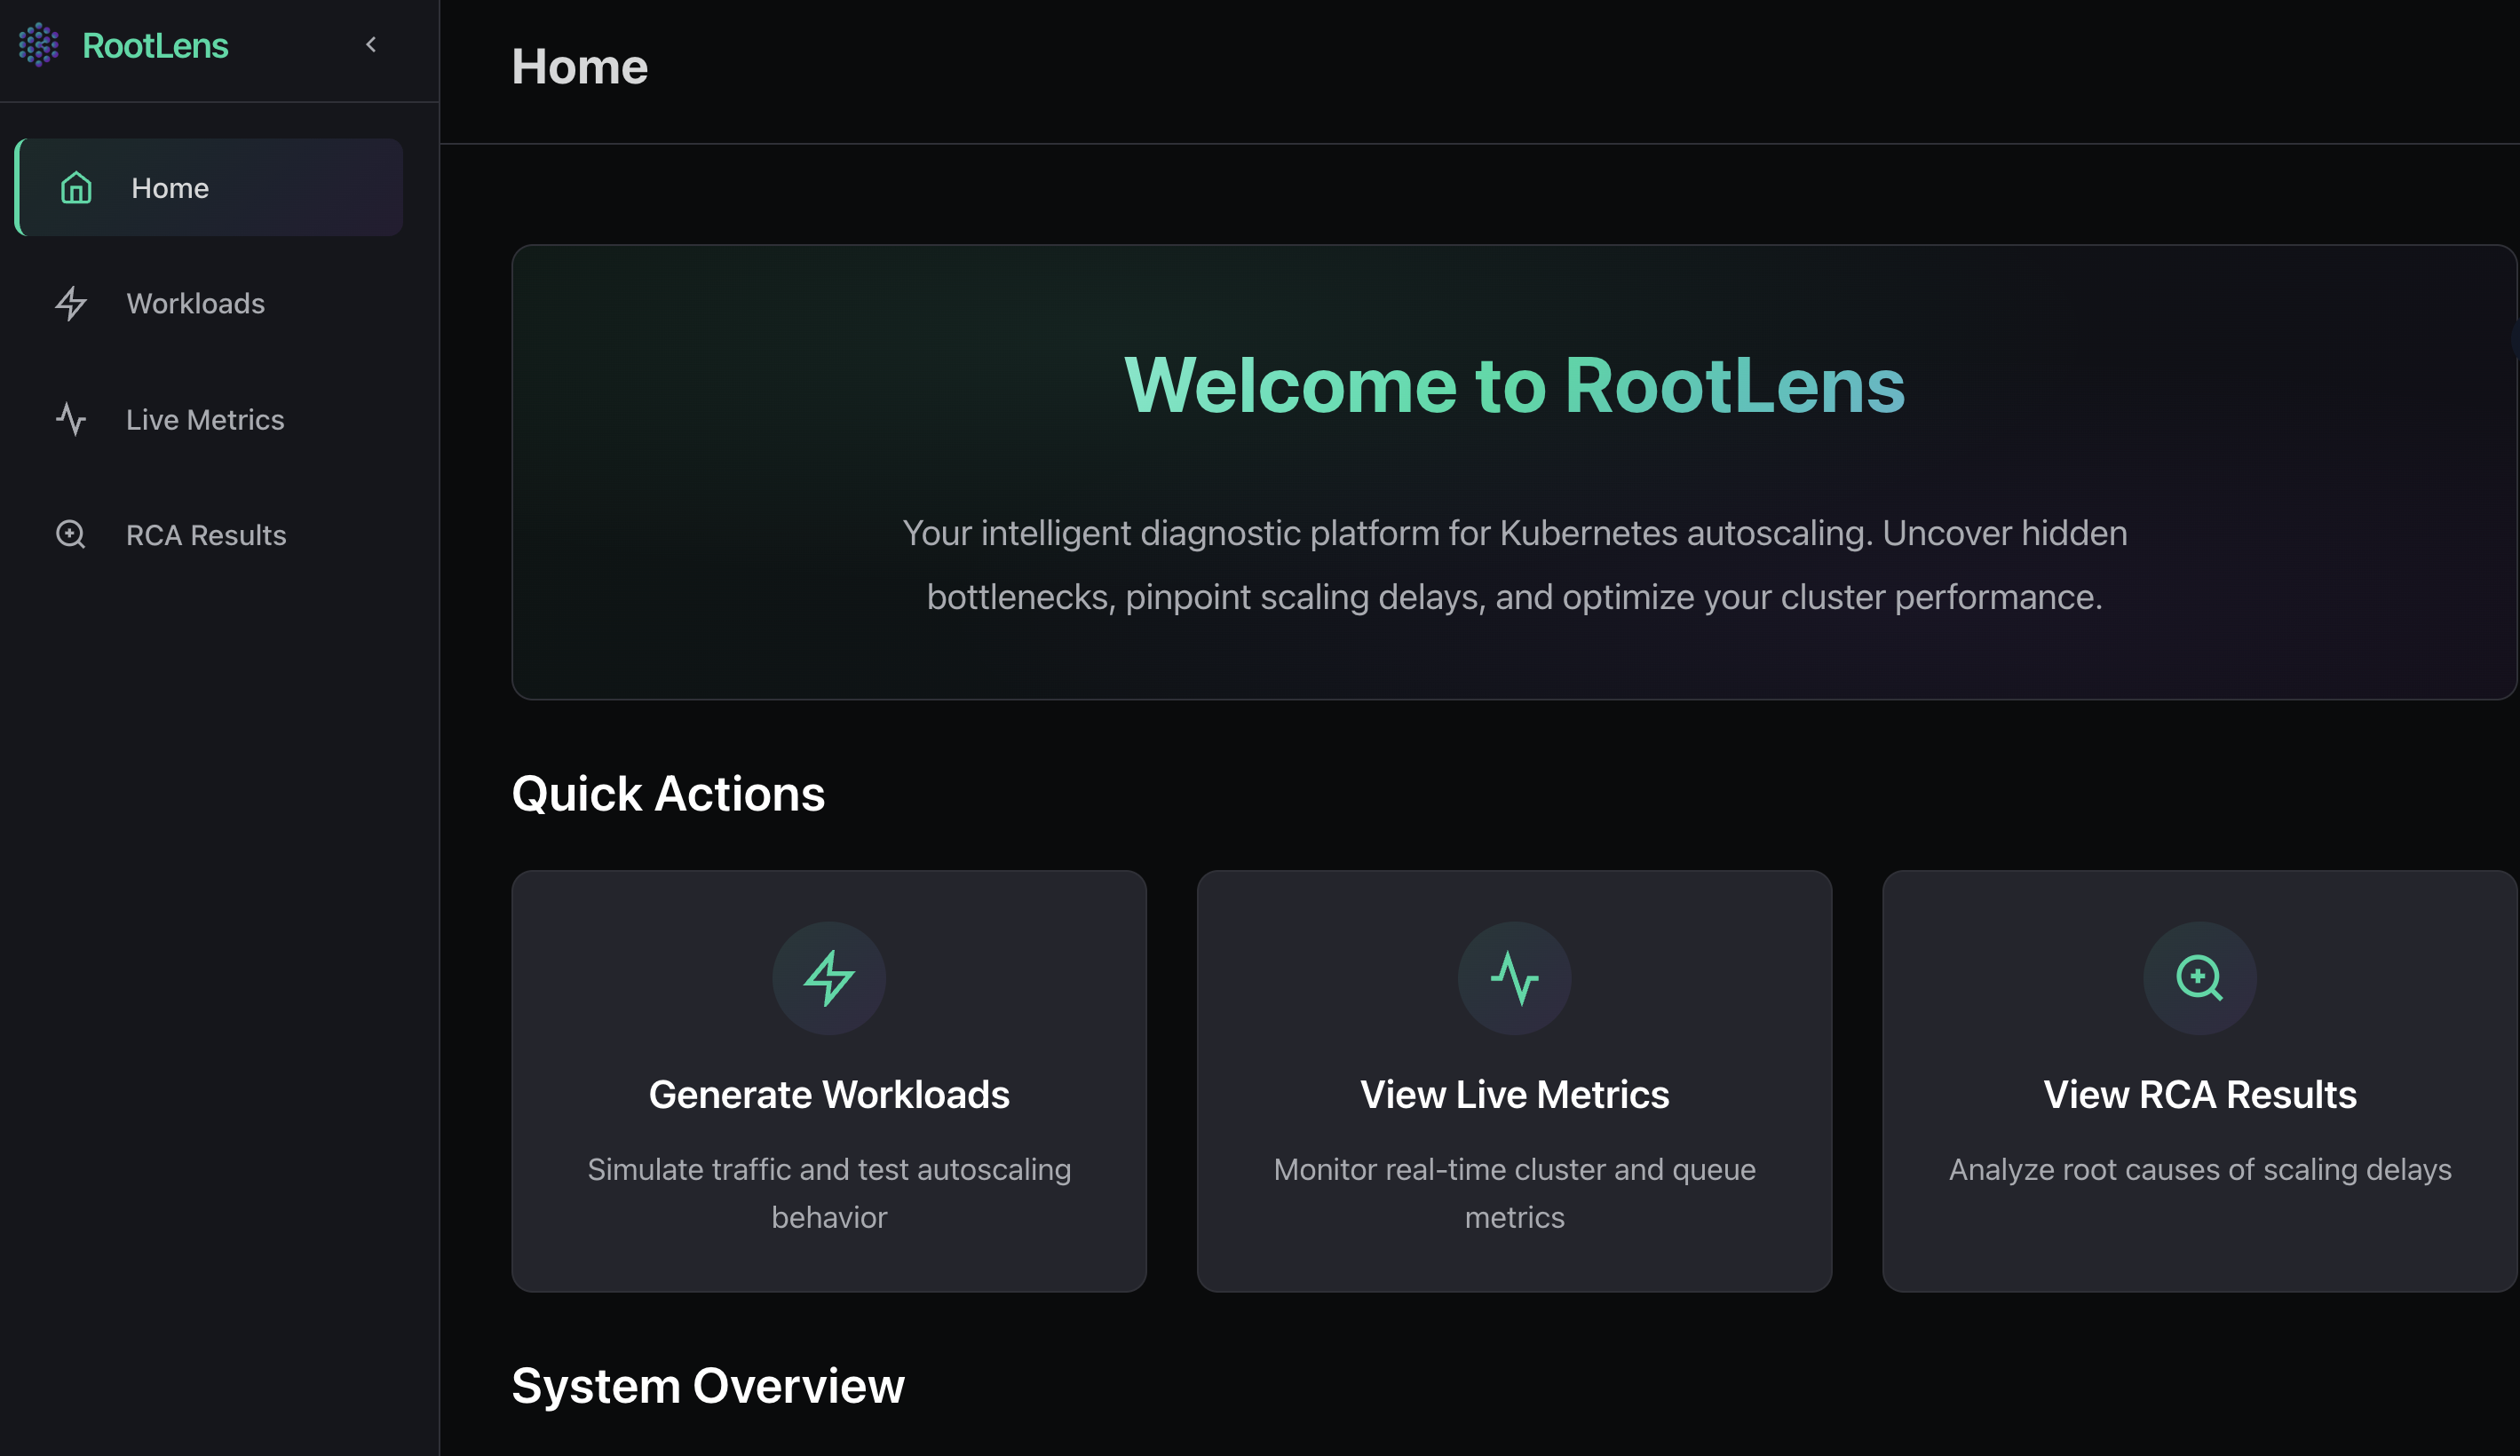
\includegraphics[width=0.95\textwidth]{thesis/assets/overview_page.png}
\caption{RootLens Dashboard: Overview Page}
\label{fig:dashboard_overview}
\end{figure}

Figure~\ref{fig:dashboard_workload} shows how to generate a workload from the dashboard.

\begin{figure}[H]
\centering
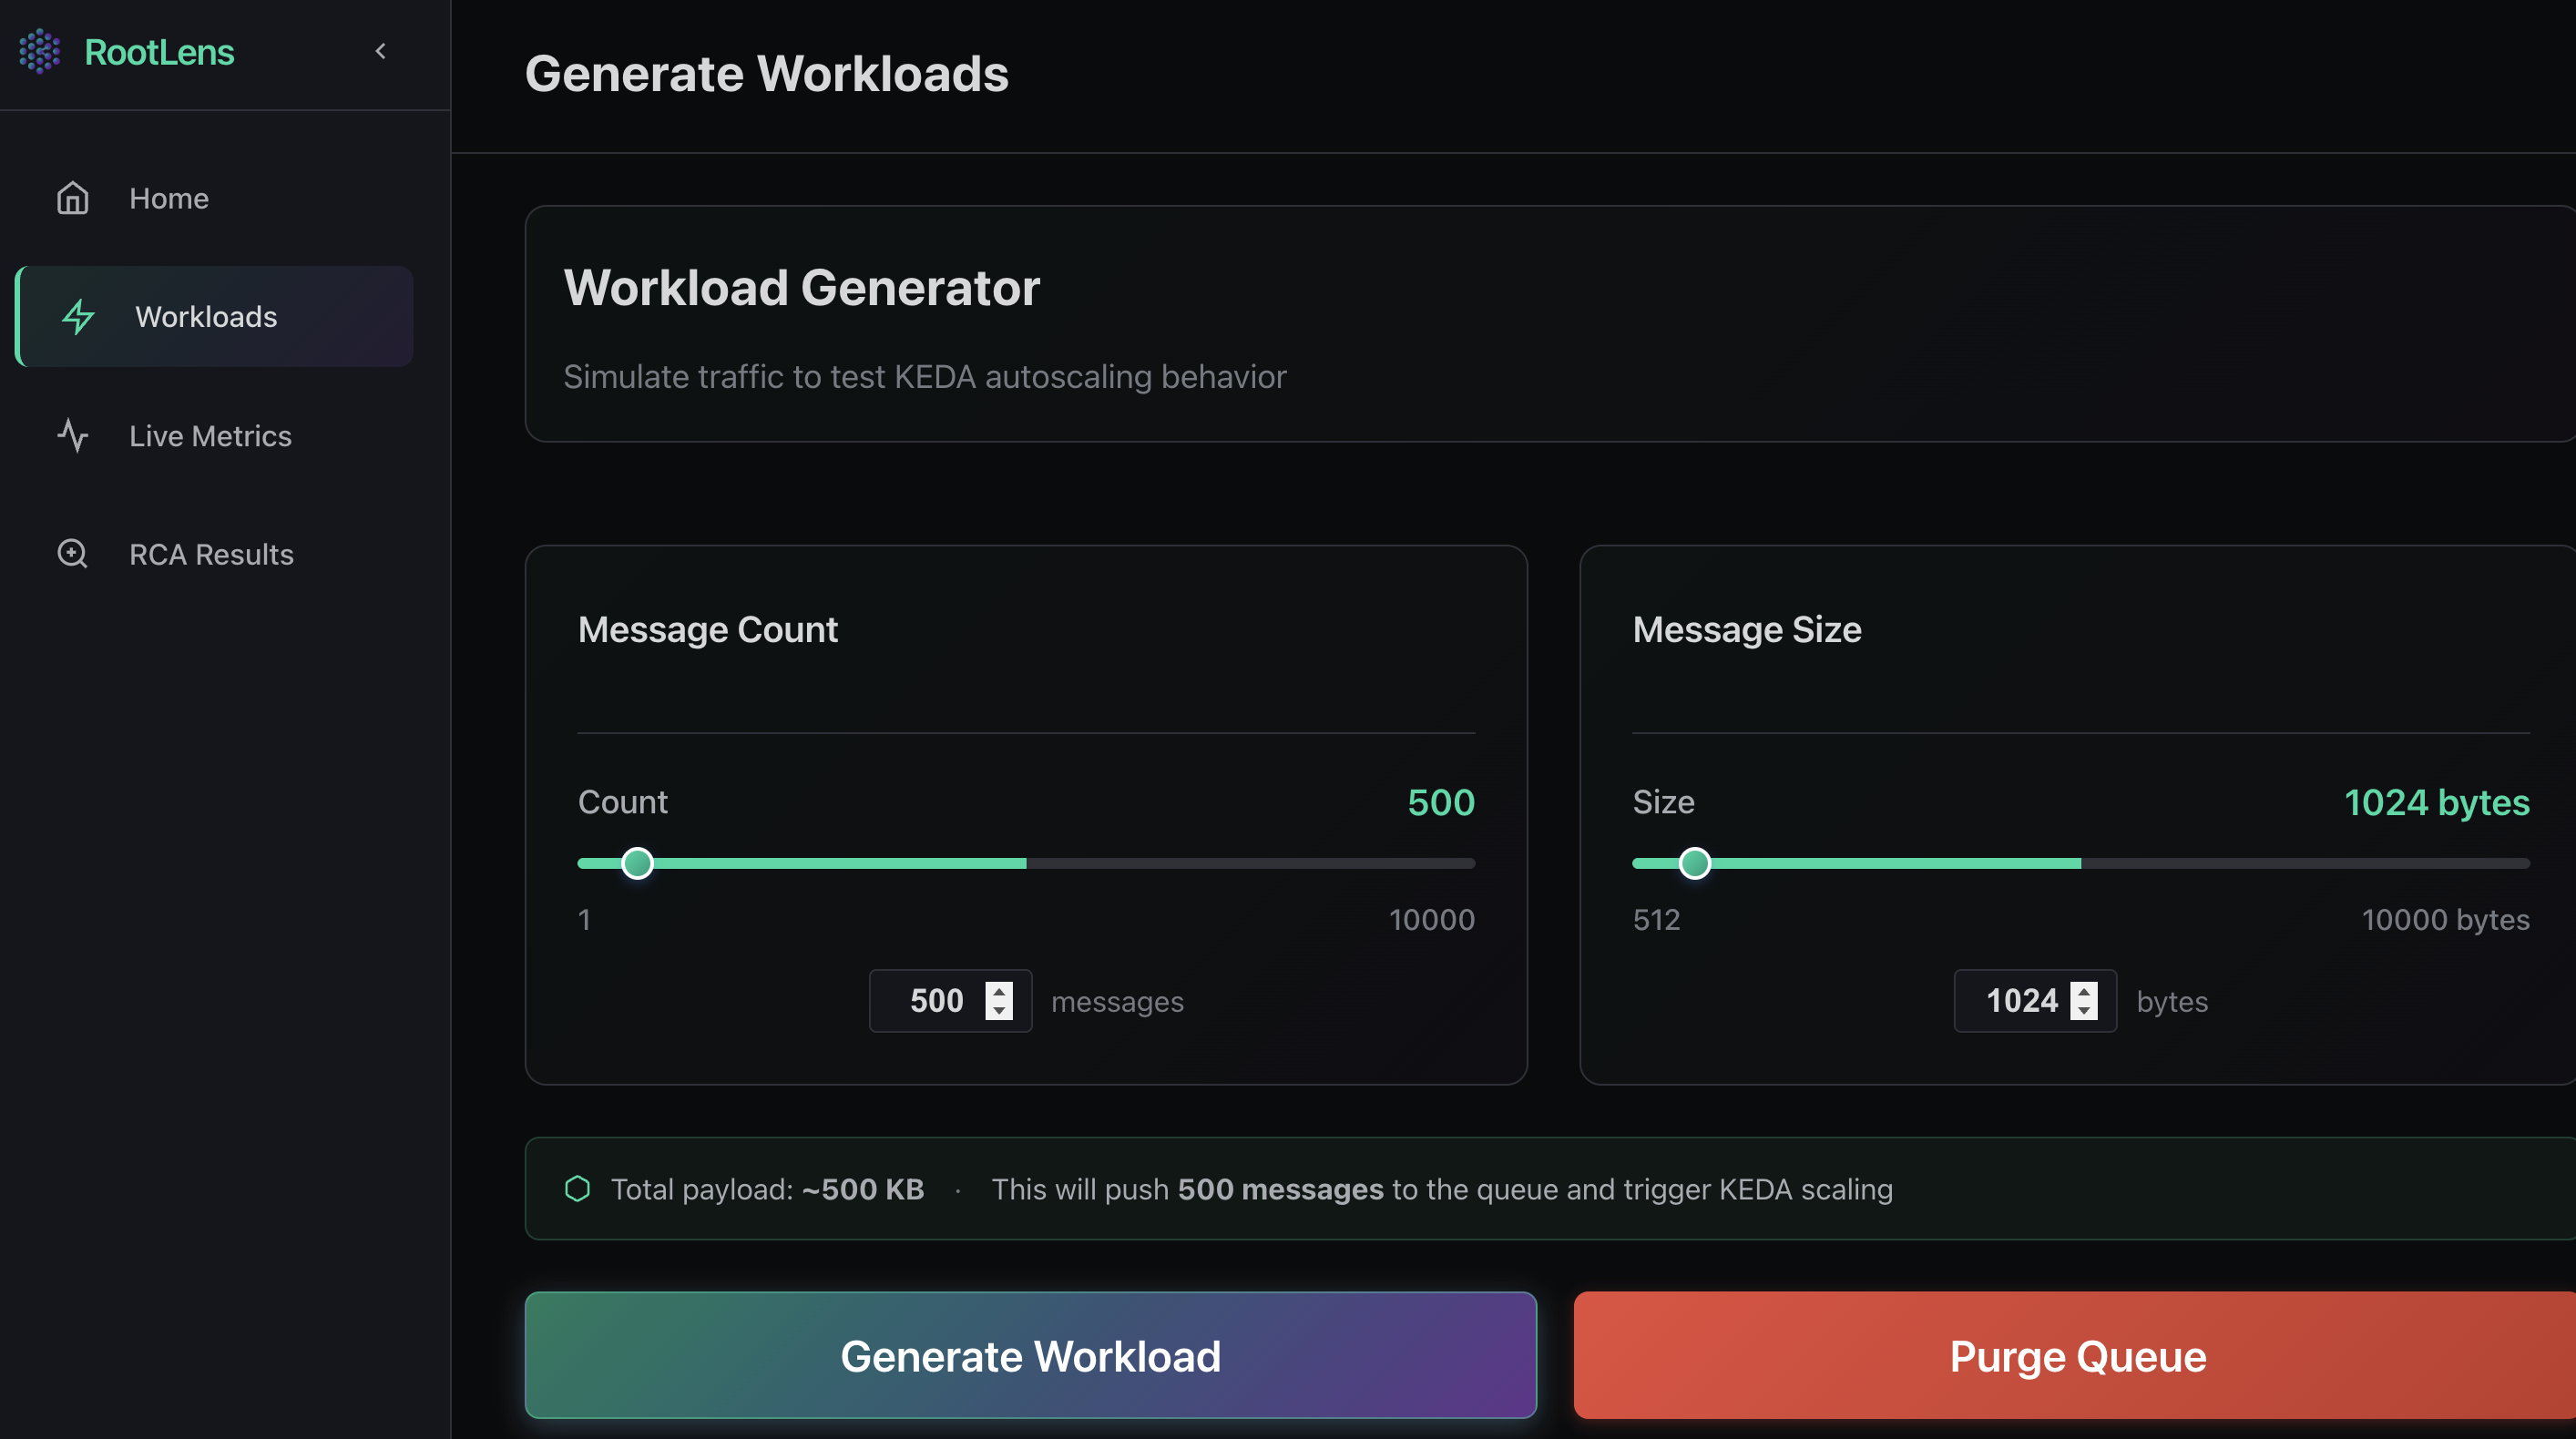
\includegraphics[width=0.95\textwidth]{thesis/assets/workload_generator_page.png}
\caption{RootLens Dashboard: Workload Generator Page}
\label{fig:dashboard_workload}
\end{figure}

Figure~\ref{fig:dashboard_metrics} shows the real-time metrics page.

\begin{figure}[H]
\centering
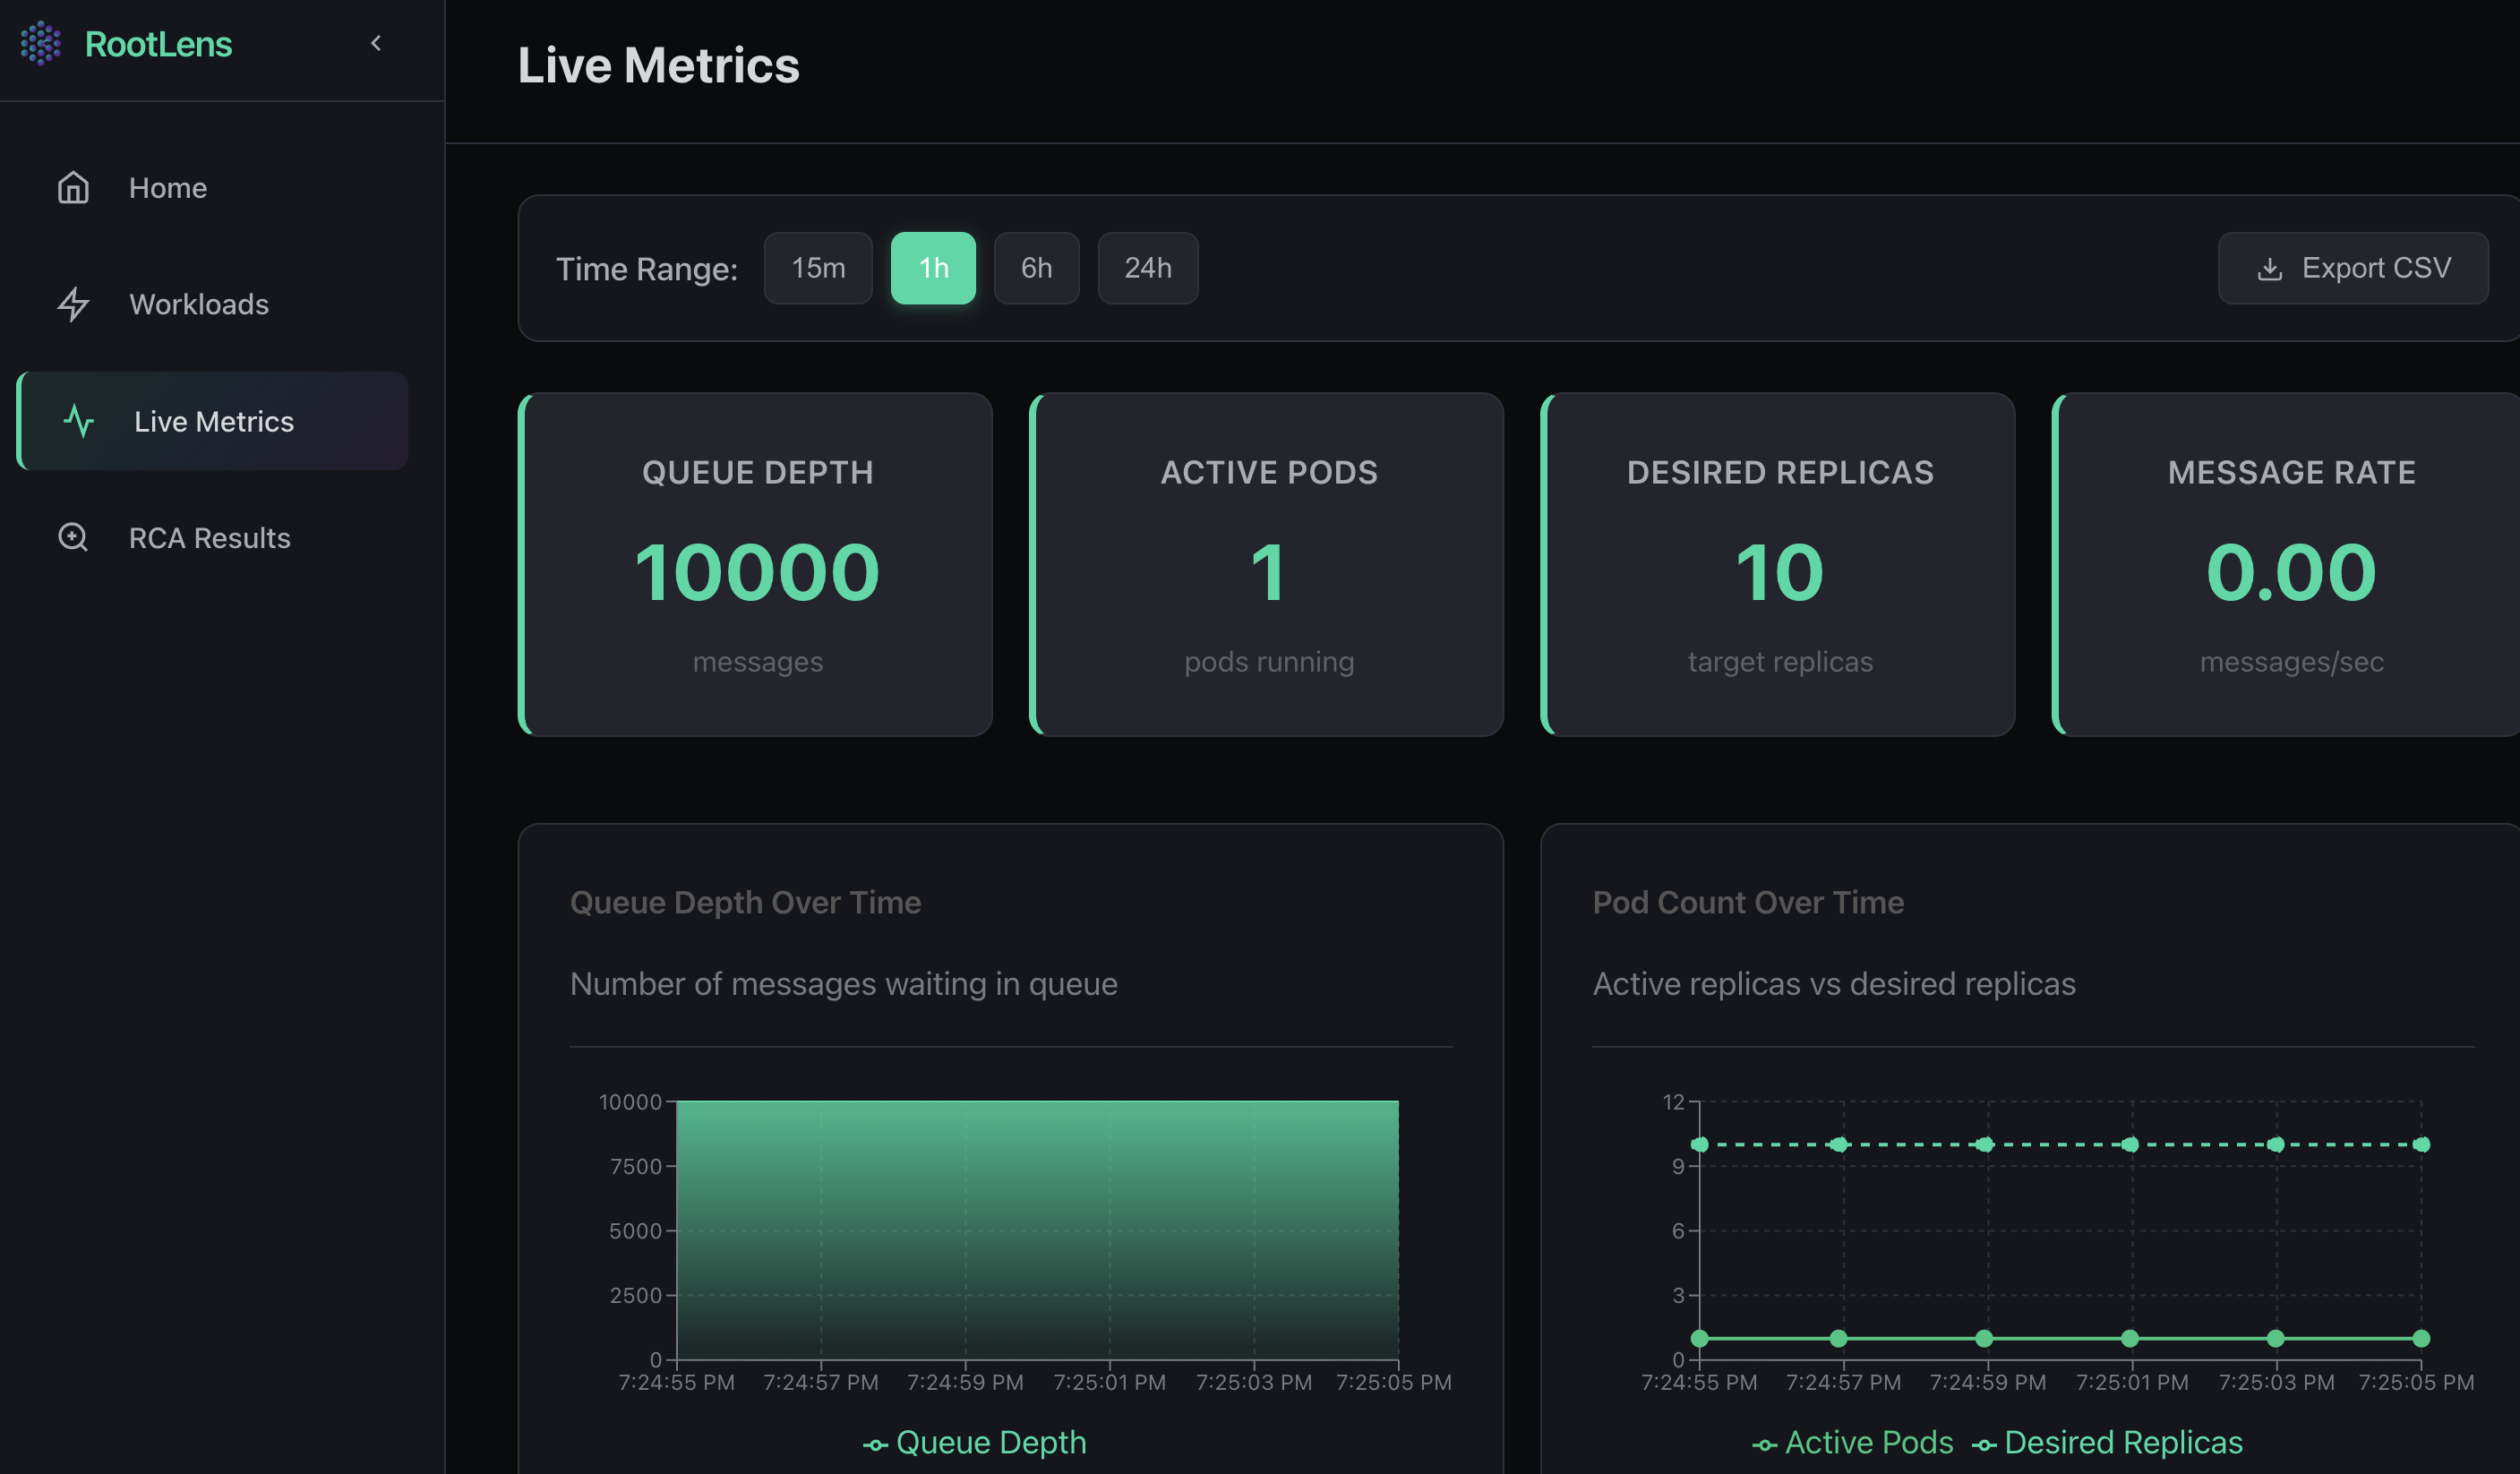
\includegraphics[width=0.95\textwidth]{thesis/assets/live_metrics_page.png}
\caption{RootLens Dashboard: Live Metrics Page}
\label{fig:dashboard_metrics}
\end{figure}

Figure~\ref{fig:dashboard_rca} shows the RCA analysis page with sub-cause probability distribution and confidence trend over recent diagnoses.

\begin{figure}[H]
\centering
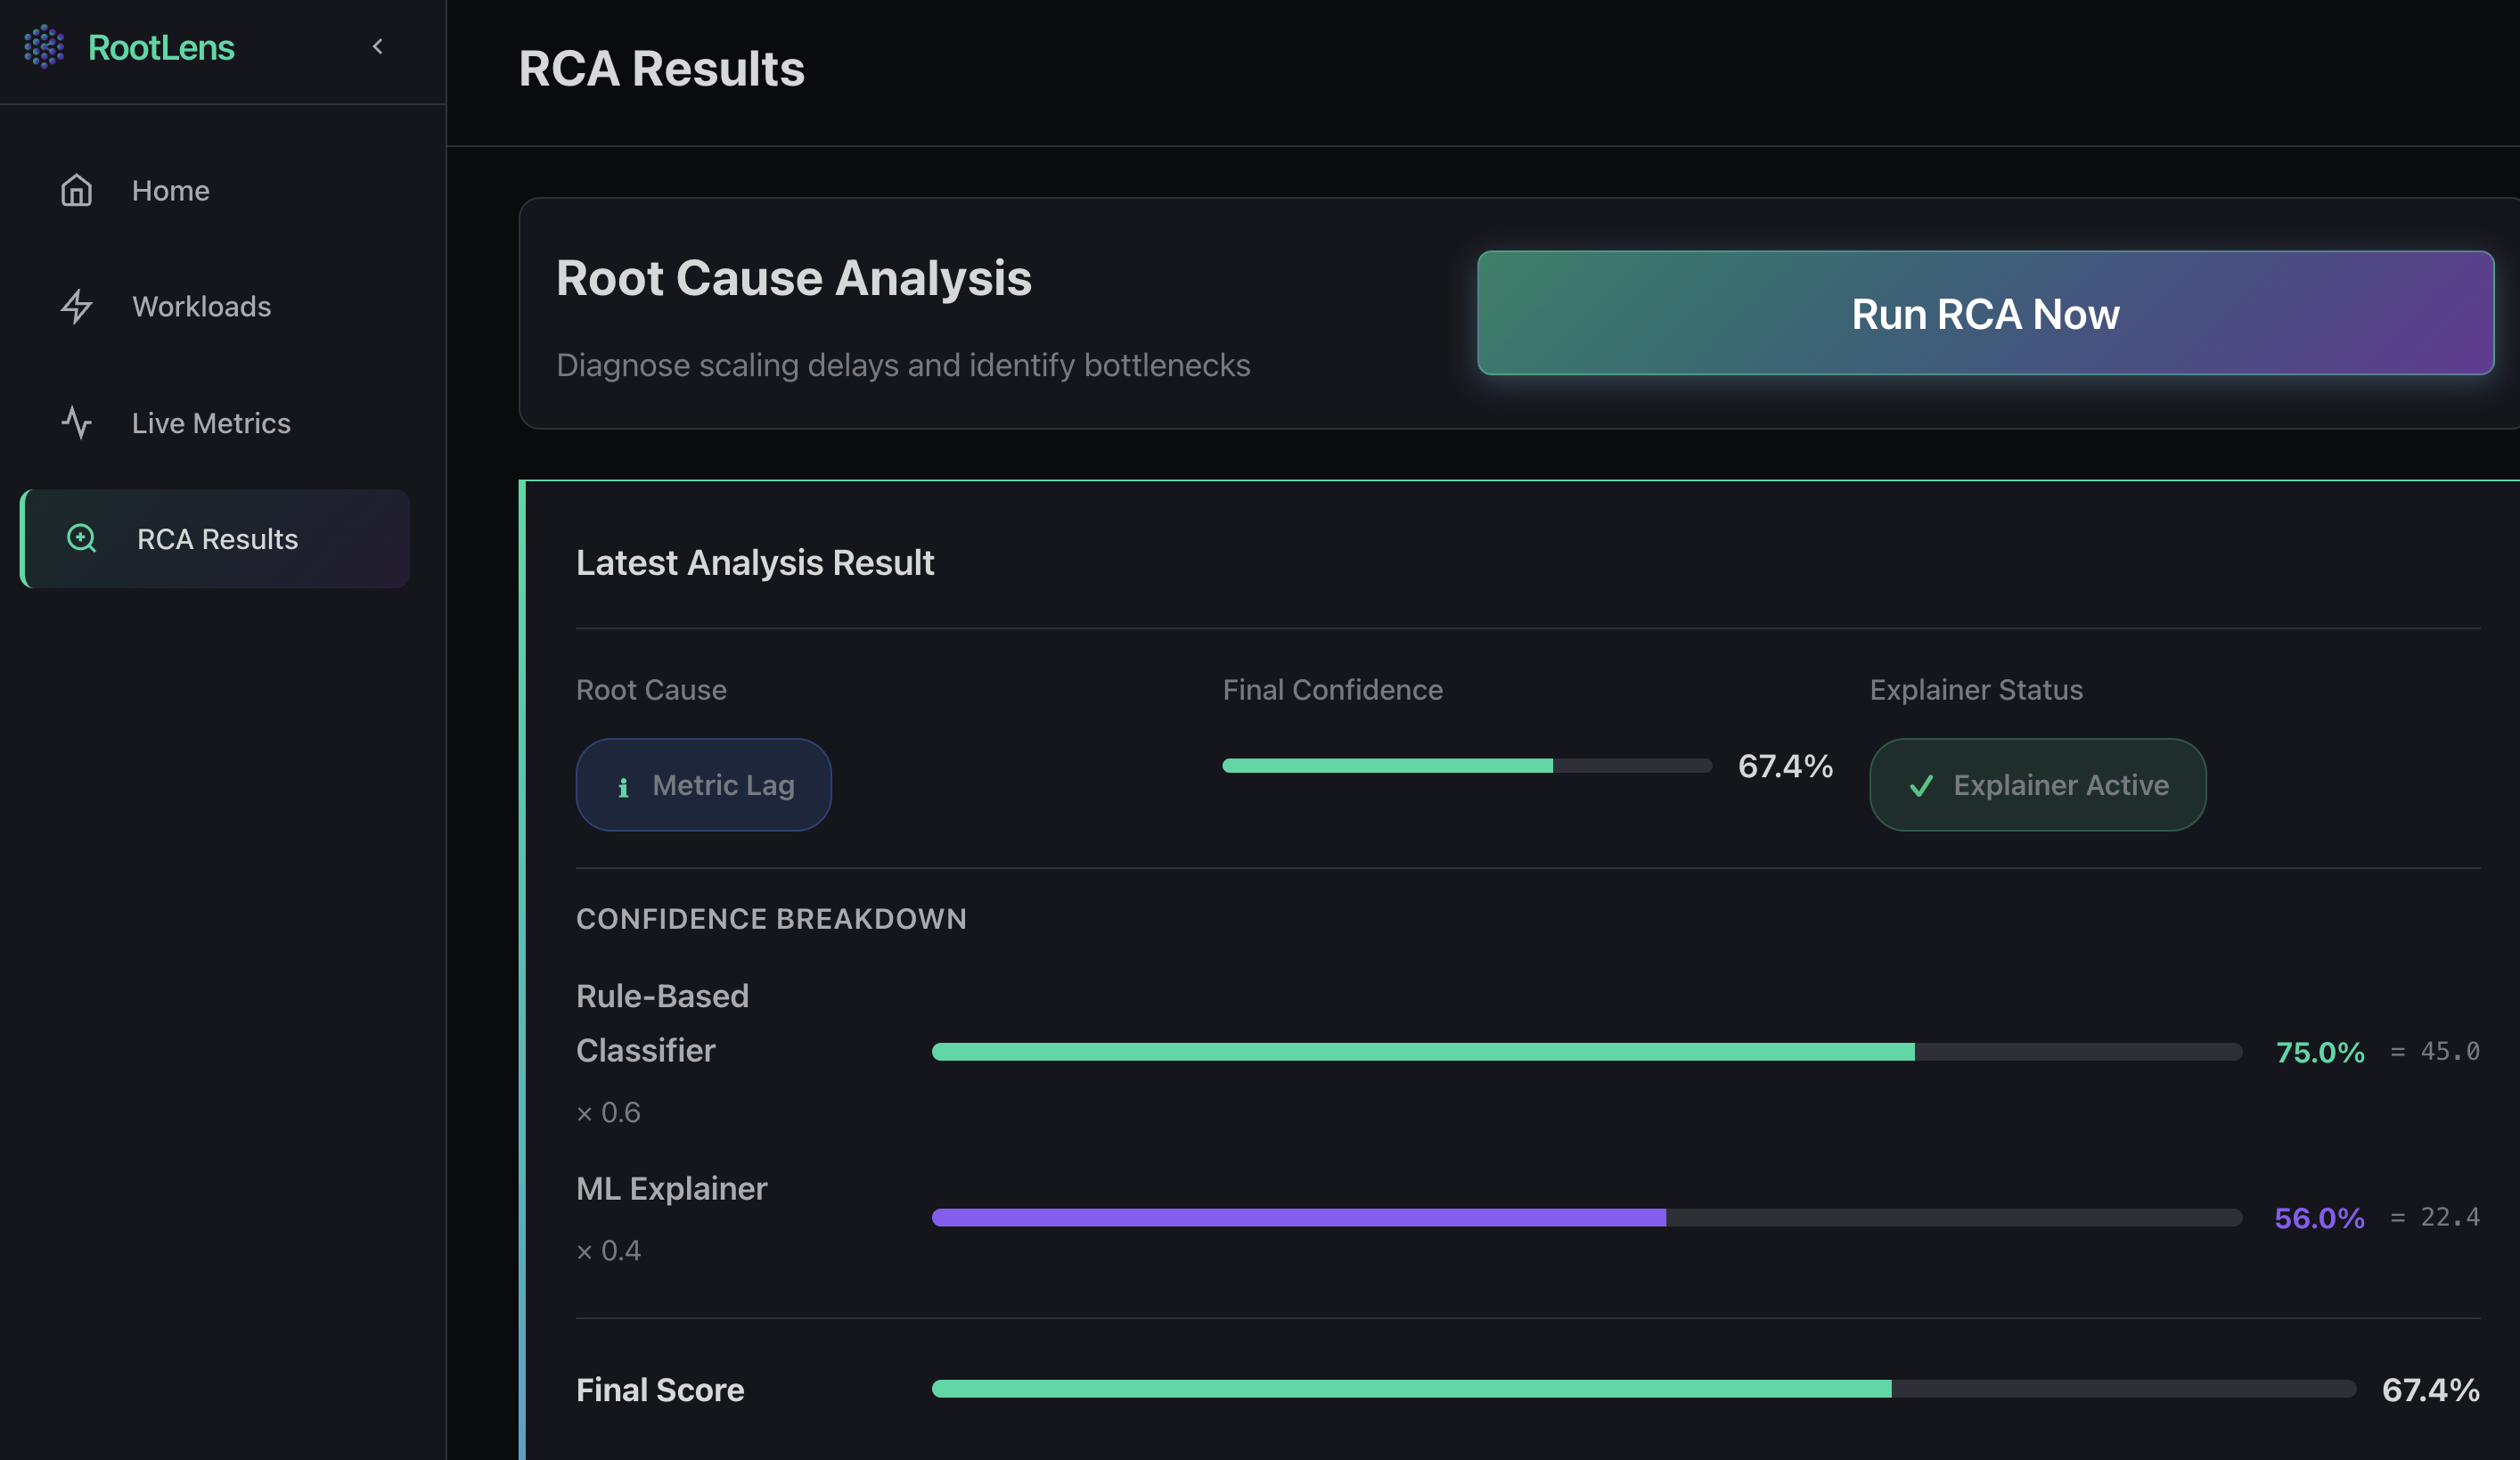
\includegraphics[width=0.95\textwidth]{thesis/assets/rca_page.png}
\caption{RootLens Dashboard: RCA Analysis Page}
\label{fig:dashboard_rca}
\end{figure}

\section{Integration of Components}
Docker Compose orchestrates all services on a shared network for local development. The Kubernetes Operator, scaffolded by kubebuilder, reconciles a single Custom Resource into the full set of Kubernetes resources required for cluster deployment. As illustrated in Figure~\ref{fig:rootlens_crd}, RootLens is deployed within the Minikube cluster as a Custom Resource Definition (CRD), enabling automated provisioning and lifecycle management of all system components.

\begin{figure}[H]
\centering
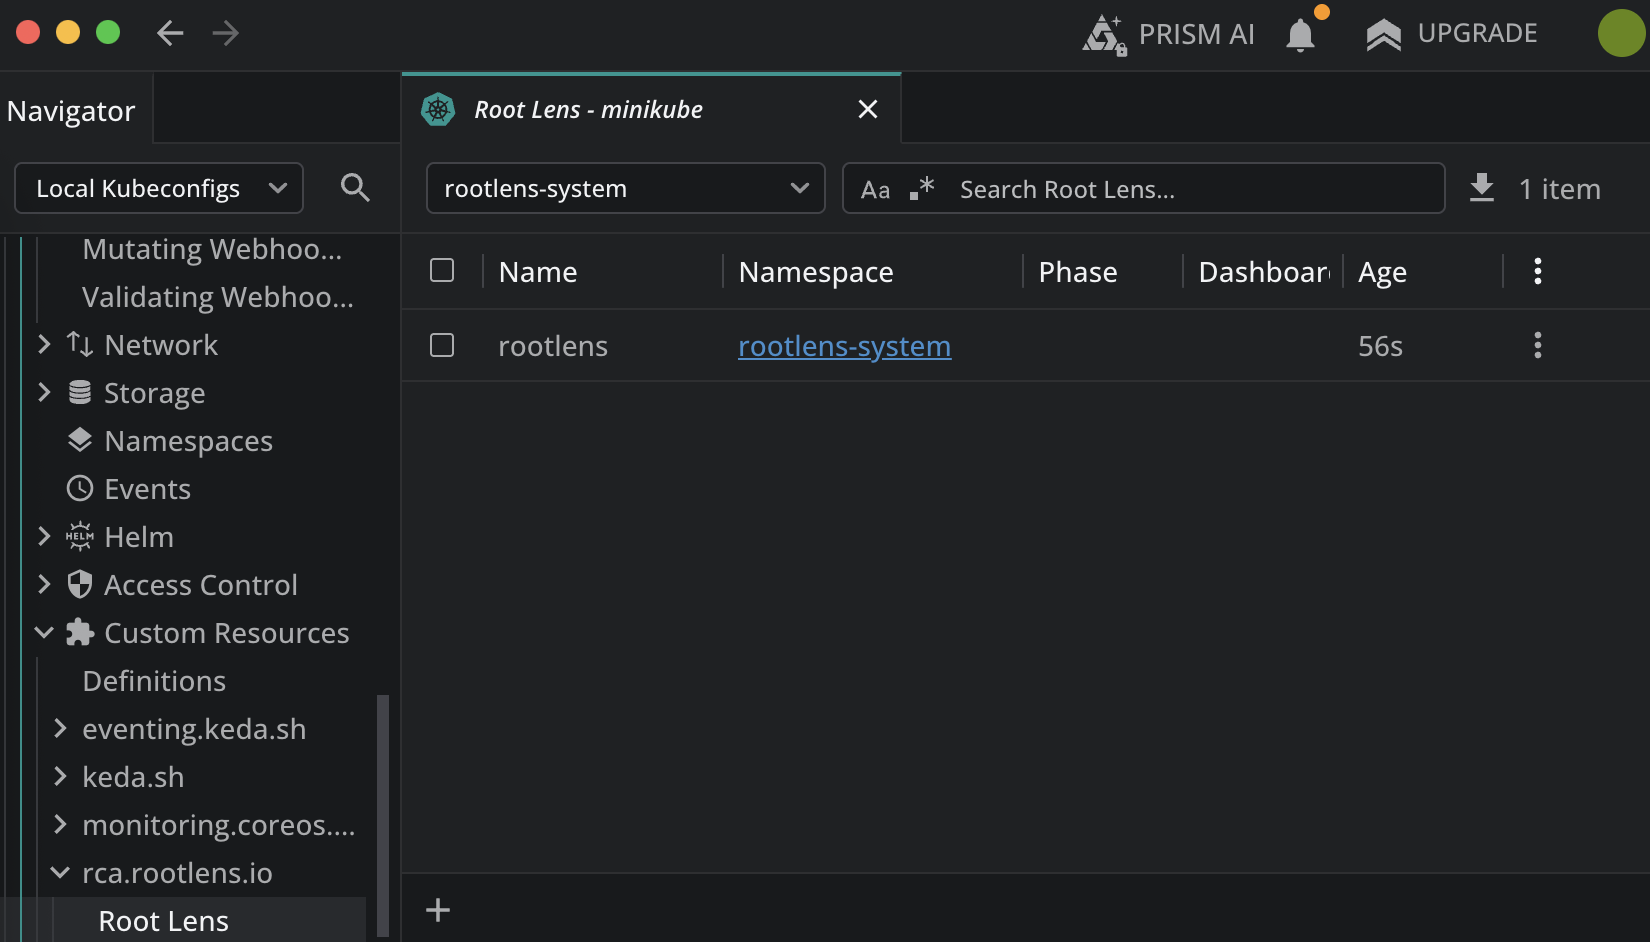
\includegraphics[width=\textwidth, height=0.6\textheight, keepaspectratio]{thesis/assets/rootlens_crd.png}
\caption{Rootlens CRD}
\label{fig:rootlens_crd}
\end{figure}

\section{Cloud Deployment}

Beyond the local Kubernetes development environment, RootLens is deployed as a production system accessible at \textbf{https://rootlens.xyz}. The three core services, the Go API backend, the React dashboard, and the Python ML inference service are deployed independently to \textbf{Google Cloud Run}, with continuous deployment orchestrated through \textbf{GitHub Actions}.

\subsection{CI/CD Pipeline}
A GitHub Actions workflow triggers on every push to the main branch. Each service has a dedicated workflow job that builds a Docker image, pushes it to \textbf{Google Artifact Registry}, and deploys the updated image to its corresponding Cloud Run service. This gives each service an independent deployment lifecycle, meaning the ML model can be updated and redeployed without restarting the Go backend. Secrets such as GCP credentials are stored as GitHub Actions secrets and injected at deploy time.

\subsection{Domain and TLS Configuration}
A custom domain was registered and DNS managed through \textbf{Cloudflare}. Domain mapping routes \textbf{rootlens.xyz} and its subdomains to the appropriate Cloud Run services. Cloudflare handles TLS termination and provides CDN caching for the static dashboard assets, while Cloud Run's managed infrastructure handles autoscaling the backend services to zero when idle.

\subsection{Operator-Based Cluster Deployment}
For teams deploying RootLens inside a Kubernetes cluster, the system is also distributable as a \textbf{Kubernetes Operator} scaffolded with kubebuilder. The Operator reconciles a single RootLens Custom Resource into the full set of Deployments, Services, and RBAC rules required to run all three components in-cluster. This dual deployment model, Cloud Run for lightweight hosted access and the Operator for in-cluster integration means RootLens can be adopted both as an external observability tool and as a native cluster component.

\section{Challenges Faced During Implementation}
Four significant implementation challenges were encountered and resolved:

\begin{enumerate}
    \item \textbf{Feature-Scaler Mismatch:} The cold start feature extractor produced 10 features while the trained scaler expected 27, causing a runtime dimension mismatch. Resolution: a formal feature contract was defined and an assertion added to validate feature count at startup.

    \item \textbf{Dashboard Always Showing ``Unknown'' Root Cause:} The storage layer was converting \texttt{EnhancedRCAResult} to \texttt{DiagnosticResult} (losing ML fields) and string constant mappings were incorrect. Resolution: storage was updated to preserve full results and constants were corrected.

    \item \textbf{Confidence Combination Not Applied:} \texttt{FinalConfidence} was copying \texttt{RuleBasedConfidence} instead of computing the weighted combination. Resolution: the combination logic was moved to a dedicated helper function called explicitly in the Classify method.

    \item \textbf{Hardcoded Credentials:} A security audit identified hardcoded credentials across eight configuration files. Resolution: all credentials replaced with environment variable references and \texttt{secretKeyRef} in Kubernetes manifests.
\end{enumerate}

\section{Technical Skills Acquired}
This project required the acquisition of several technical competencies beyond the undergraduate curriculum. \textbf{Kubernetes Operator development} using kubebuilder and the controller-runtime library required learning custom resource definition design, reconciliation loop patterns, and Kubernetes RBAC configuration. \textbf{ML engineering}, including feature contract management across Go and Python language boundaries, scaler synchronisation, and model versioning with wrapper dictionaries, was developed through iterative debugging of the cross-service integration. \textbf{Chaos engineering methodology} (Basiri et al., 2016) was learned and applied to design the fault-injection experimental protocol. \textbf{Cross-language service integration}, designing and maintaining a stable HTTP JSON contract between Go and Python services with independent deployment lifecycles, required practical experience in API contract design and defensive error handling.

\section{Contribution to Practice}
The implementation demonstrates that a hybrid rule-ML root cause analysis system for Kubernetes autoscaling delays can be built and evaluated with sub-200ms end-to-end latency on a single-node development cluster. The Go and Python microservice architecture, with its well-defined HTTP JSON contract and graceful degradation path, provides a reusable architectural template for integrating ML inference into latency-sensitive operational tooling. The category-specific explainer routing pattern, where the rule-based engine selects which ML model to invoke based on its primary classification, is a novel integration strategy that avoids the complexity of a monolithic multi-class classifier while maintaining sub-cause granularity.

\section{Chapter Summary}
This chapter described the implementation of RootLens across its core components: concurrent goroutine-based data collection from Kubernetes, KEDA, and RabbitMQ; the rule-based RCA engine with threshold classification and confidence scoring in Go; the ML explainer service with category-specific Random Forest models served via Flask; and the React dashboard providing real-time visualisation. The Go-Python integration via HTTP JSON contracts, the model loading pipeline with wrapper-handling logic, and the chaos engineering dataset generation methodology were presented. Four significant implementation challenges and their resolutions were documented, demonstrating practical engineering lessons in cross-language ML integration. Chapter~8 presents the testing and evaluation of the completed system.
